%!TEX root = ../thesis.tex

% \vspace{-10pt}

\section{本章の概要}
本章では,\ref{sec:oculus-exp-overview}節で実験の概要を示す.また,\ref{sec:oculus-exp-method}節で実験方法,\ref{sec:oculus-exp-result}節で結果と考察について述べる.

\section{実験概要}\label{sec:oculus-exp-overview}
提案手法の有効性を評価するために,現実の環境においてロボットと歩行者がどのように相互作用するかを観察し,提案手法を用いてその行動を予測する実験を行う.実験には20代の男性4名が参加し,その中からランダムに選ばれた2名のデータを予測用に利用した.

\section{実験方法}\label{sec:oculus-exp-method}
本実験は丹野らの研究\cite{si2023-tanno}を参考にして実施したものである.実験は\figref{Fig:oculus-exp-overview}に示す室内環境で行い,\figref{fig:tracking-robot}に示す移動ロボット(ORNE-box2\cite{井口颯人2023屋外自律移動ロボットプラットフォーム-orne})を使用した.実験参加者は\figref{Fig:oculus-exp-overview}に示したように,移動ロボットの正面から歩行を開始し,事前に指定された目的地(A/B/C)のいずれかまでロボットを避けながら歩行する.各参加者には,各目的地への歩行を3回ずつ繰り返してもらった.ロボットの行動が歩行者の将来の軌道にどのように影響するかを観察するため,ロボットは一定の速度0.3m/sで直進した後,次の3つの挙動のいずれかを事前に知らせることなく実行する.

\begin{itemize}
  \item 速度を変えず直進
  \item 速度を変えず右に避ける
  \item 速度を変えず左に避ける
\end{itemize}

\figref{fig:tracking}に示すように,参加者とロボットの位置はOculus Riftの専用コントローラを用いて計測する.また,正確にコントローラをトラッキングするため,2基の赤外線センサを\figref{Fig:oculus-exp-overview}の斜線部に\figref{Fig:oculus-sensor}のように配置する.データは,ETH\cite{pellegrini2009you-eth},UCY\cite{lerner2007crowds-ucy}データセットのフォーマットで取得する.

予測の評価は,\ref{chap:proposed_method}章で行った予備実験と同じ手順で進めた.ロボットの行動を考慮した軌道予測手法の有効性を評価するため,ロボットの行動を考慮する場合としない場合の予測を行い,それぞれの結果を比較する.

\begin{figure}[H]
  \centering
 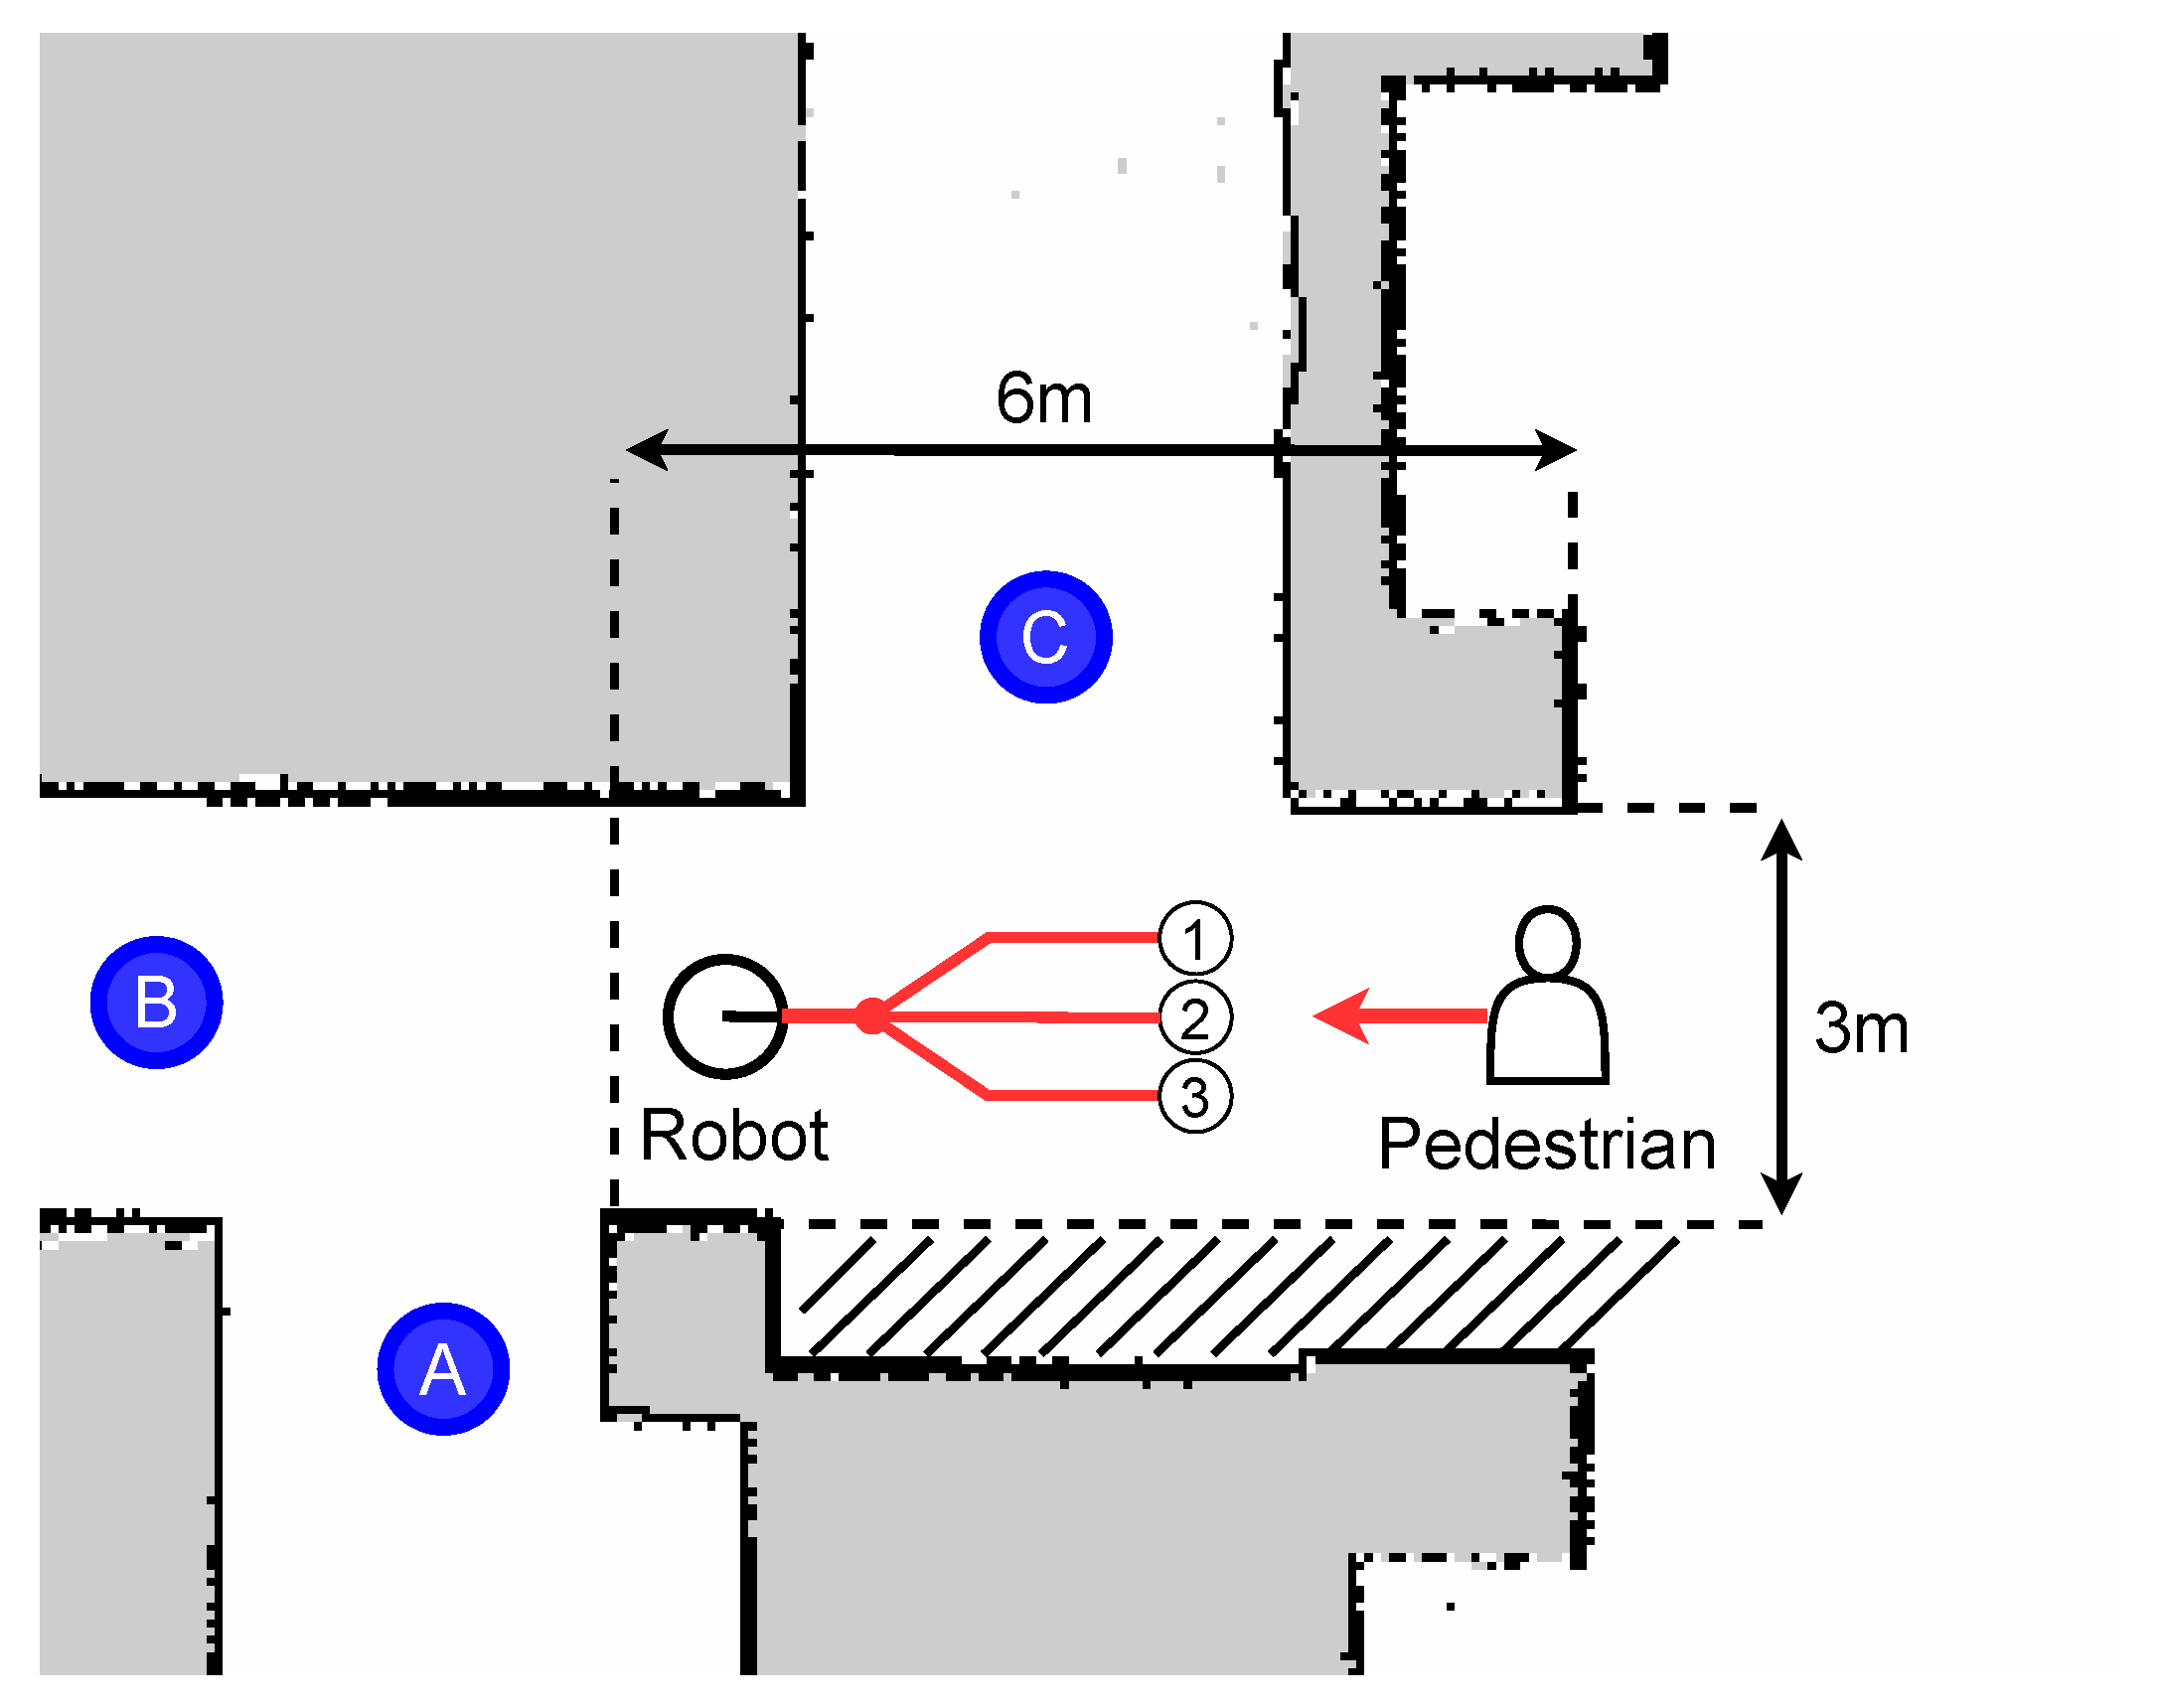
\includegraphics[keepaspectratio, scale=0.27]
      {images/oculus_experiments.pdf}
\caption{Experimental environment}
 \label{Fig:oculus-exp-overview}
\end{figure} 

\begin{figure}[H]
  \centering
  \begin{minipage}{0.42\textwidth}
    \centering
    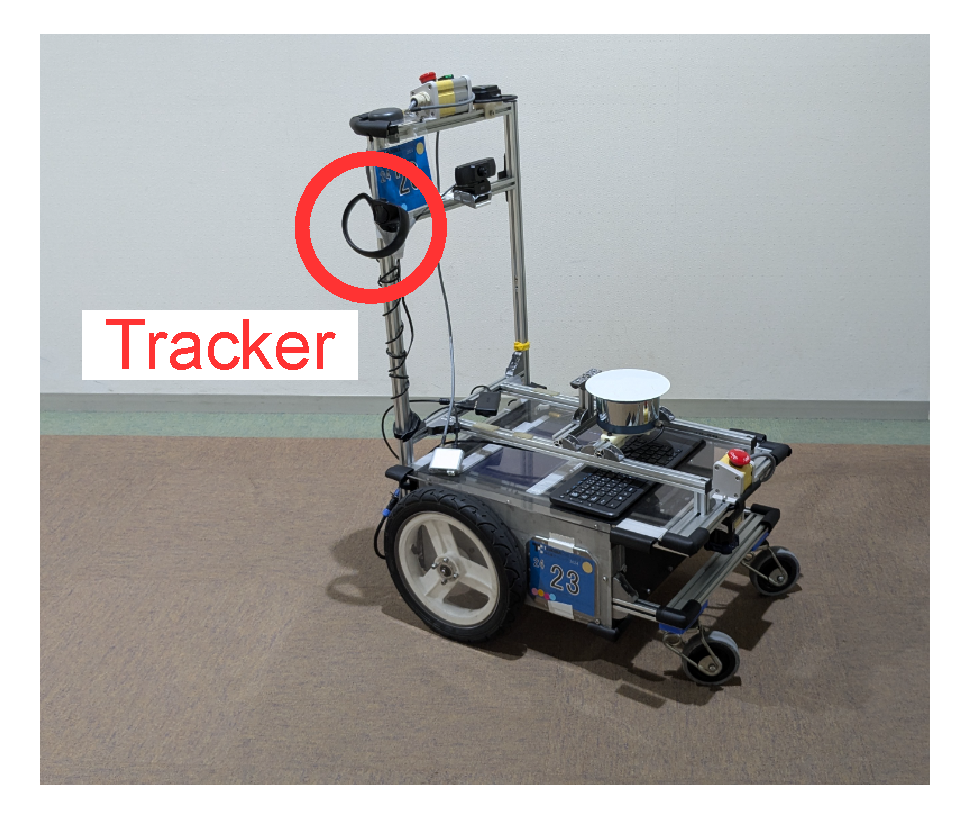
\includegraphics[width=\textwidth]{images/tracking-robot.pdf}
    \subcaption{Robot}
    \label{fig:tracking-robot}
  \end{minipage}
  % \hfill
  \begin{minipage}{0.42\textwidth}
    \centering
    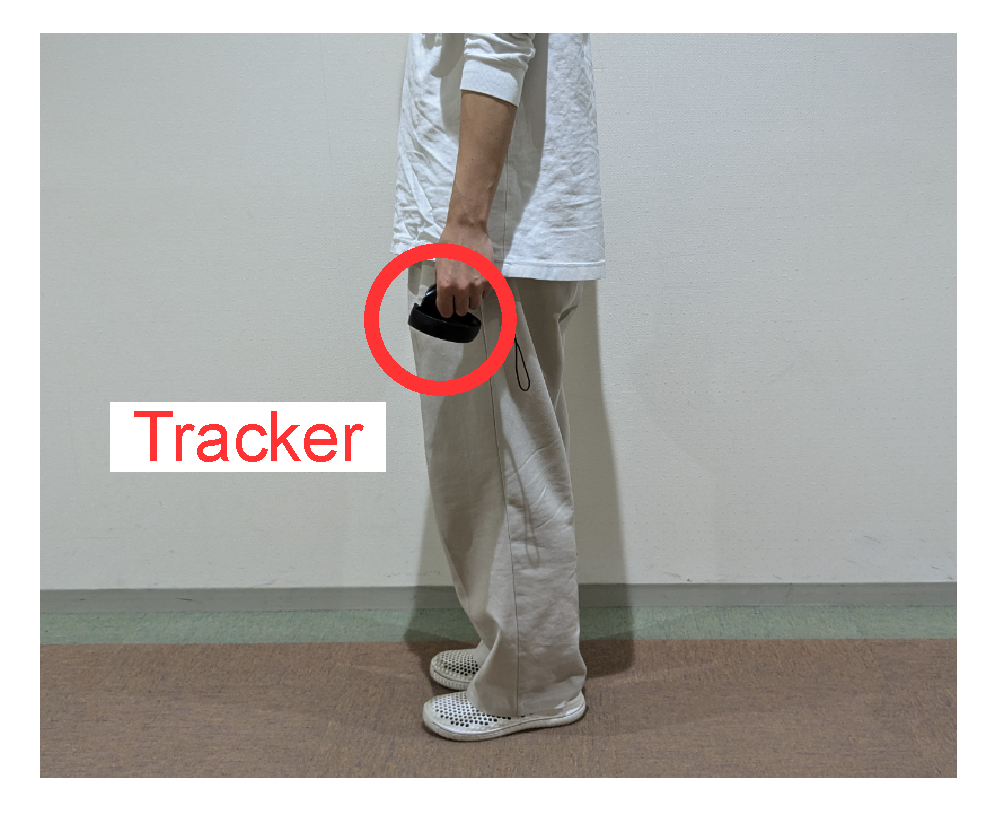
\includegraphics[width=\textwidth]{images/tracking-ped.pdf}
    \subcaption{Pedestrian}
    \label{fig:tracking-ped}
  \end{minipage}
  \caption{Tracking sensor setup}
  \label{fig:tracking}
\end{figure}

\vspace{-20pt}

\begin{figure}[H]
  \centering
 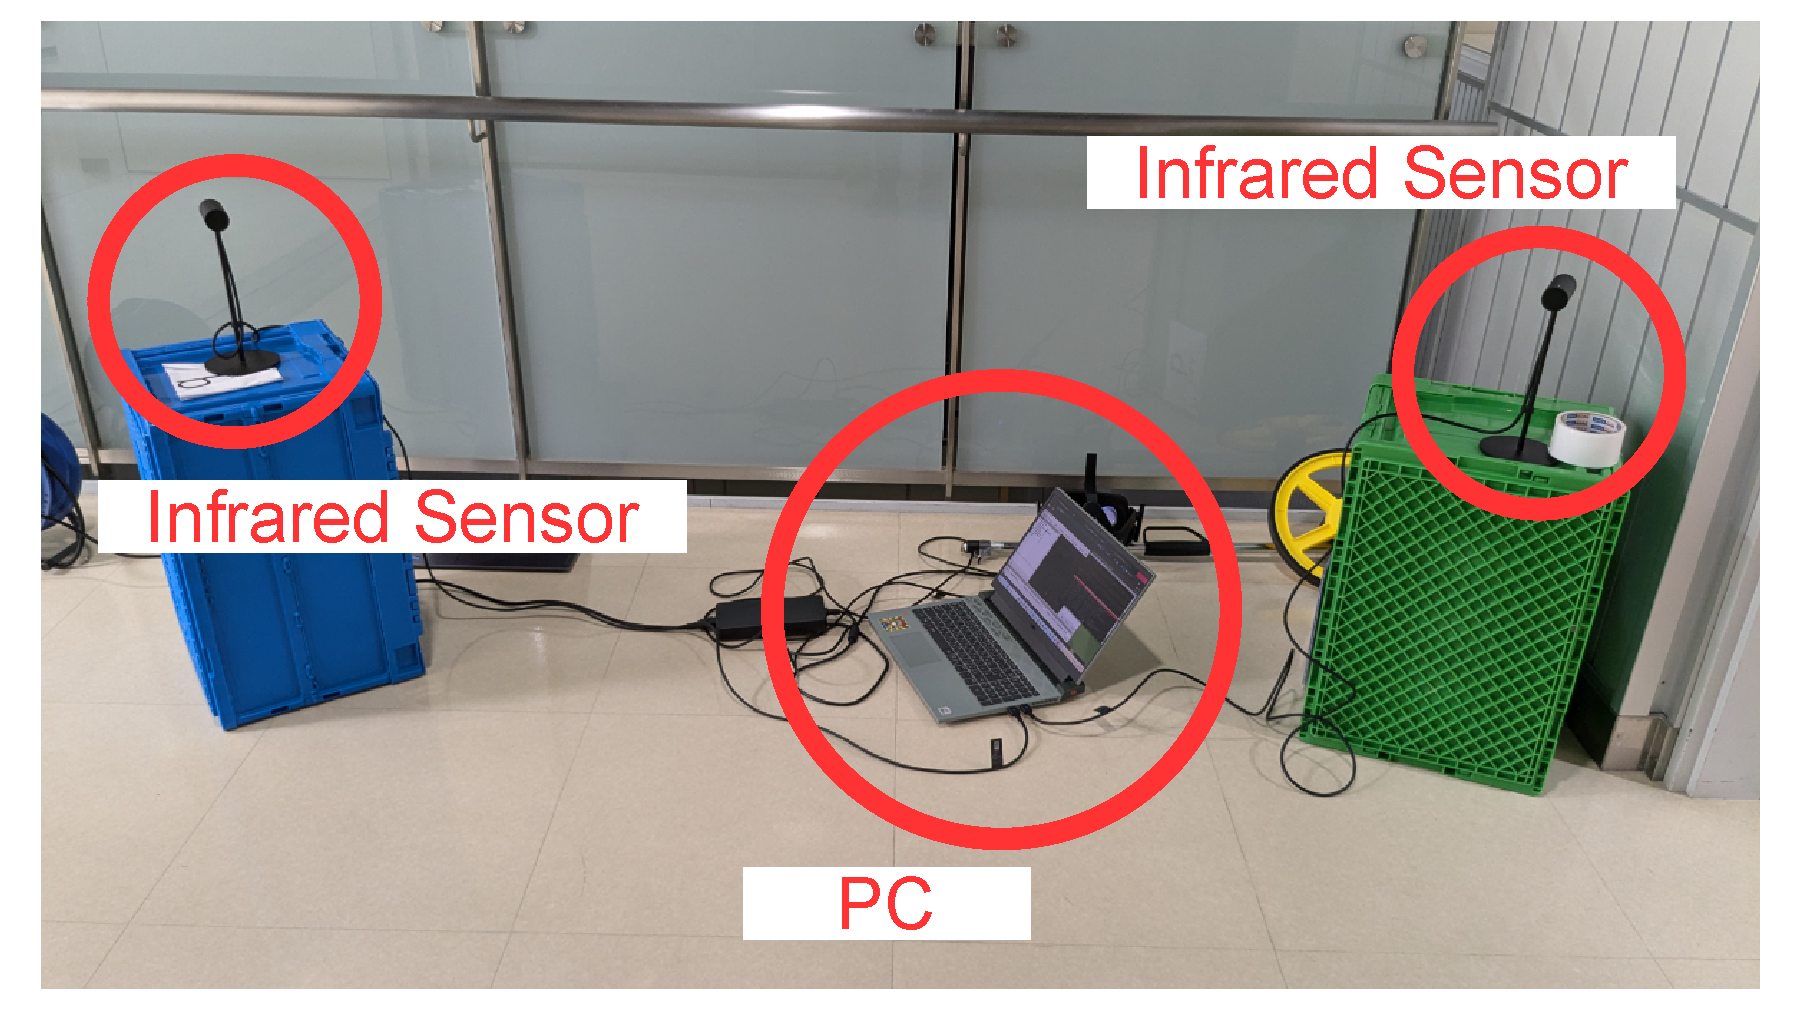
\includegraphics[keepaspectratio, scale=0.32]
      {images/tracking-sensor.pdf}
\caption{Infrared sensor setup}
 \label{Fig:oculus-sensor}
\end{figure}

\vspace{-20pt}

\section{結果と考察}\label{sec:oculus-exp-result}
\tabref{tab:robot-behavior}に,ロボットの行動を考慮する場合としない場合における各評価指標の値を示す.考慮しない場合に比べて,ADEは7.5%,FDEは15.9%誤差を改善した.
この結果から,ロボットの行動を考慮することで,歩行者の軌道予測の精度が向上することがわかる.特に,FDEの改善が顕著であり,これはロボットの動きが歩行者の最終的な位置に大きな影響を与えることを示唆している.一方で,ADEの改善は比較的小さい.これは,\figref{Fig:oculus-exp-overview}に示したように,3箇所の目的地の内,2箇所で角を曲がる必要があるため,途中の軌道予測が困難であり,評価指標の値の改善が抑えられたと考えられる.

\begin{table}[H]
  \begin{center}
  \caption{Comparison with and without taking into account the robot's behavior}
  \label{tab:robot-behavior}
  % \footnotesize
  \begin{tabular}{c||c|c}
   & ADE & FDE \\ 
  \hline \hline
  Normal      & 0.40       & 0.69                      \\
  \hline
  Considering robot behavior    & 0.37       & 0.58                      \\
  \hline
  \end{tabular}
  \end{center}
\end{table}

\figref{Fig:pred-straight},\figref{Fig:pred-right},\figref{Fig:pred-left}に実験で取得した目的地Aへの歩行データに対する予測例を示す.この予測例は,ロボットが行動を取り始める時刻を最終観測時刻とした.ロボットの行動を考慮せず予測を行うと,いずれのロボットの行動に対しても避けるような予測は見られなかった.
一方,ロボットの行動を考慮した予測では,より真値に近い予測を行う様子が確認できた.
観測時間内では,人間の行動は一貫して直進しているため,その後のロボットを避けるような予測は困難であるが,\figref{Fig:pred-straight},\figref{Fig:pred-right}では,ロボットを避けるような予測をしている.このことから,ロボットの行動を考慮した軌道予測は,人間とロボット間の相互作用を捉えていることが分かる.

\vspace{-10pt}

\begin{figure}[H]
  \centering
 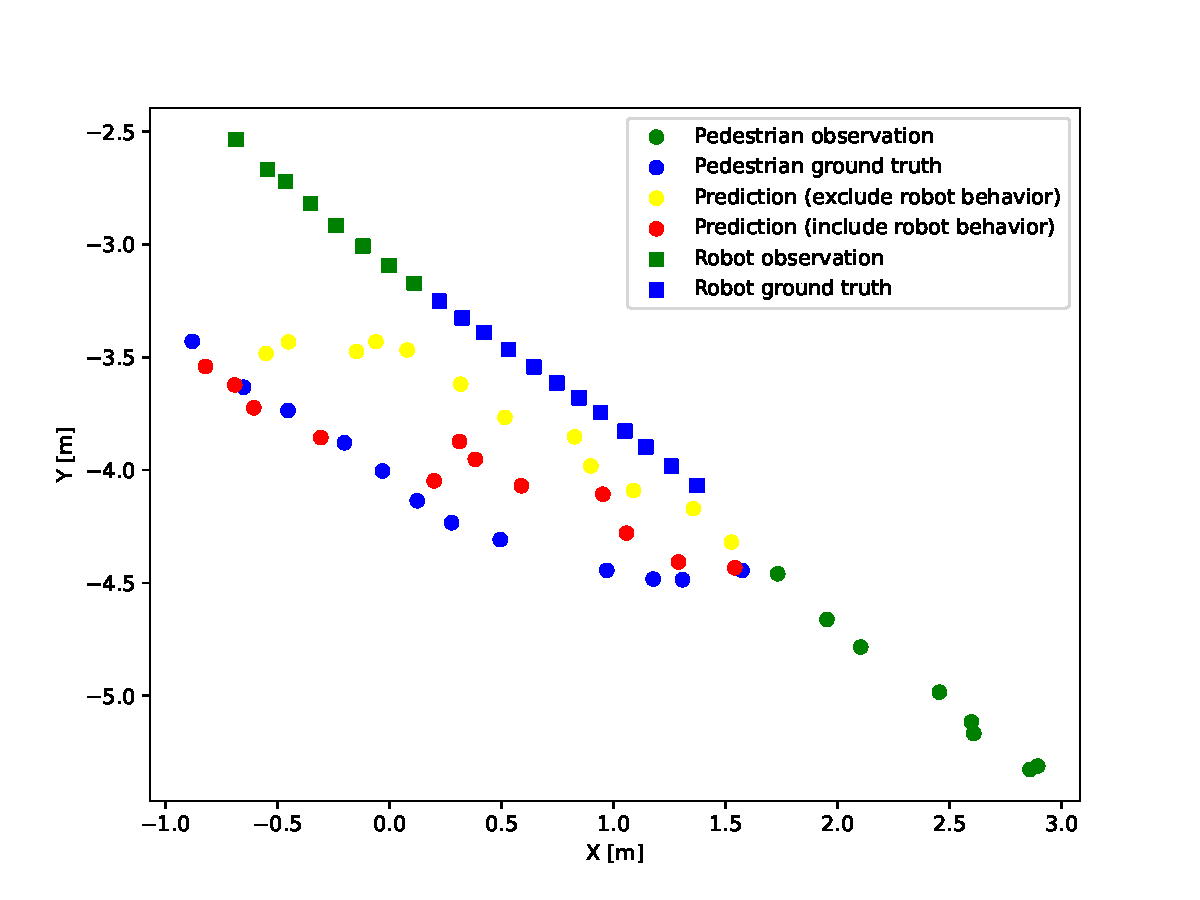
\includegraphics[keepaspectratio, scale=0.58]
      {images/pred_straight.pdf}
\caption{Predicted trajectory when the robot moves straight}
 \label{Fig:pred-straight}
\end{figure}

\begin{figure}[H]
  \centering
 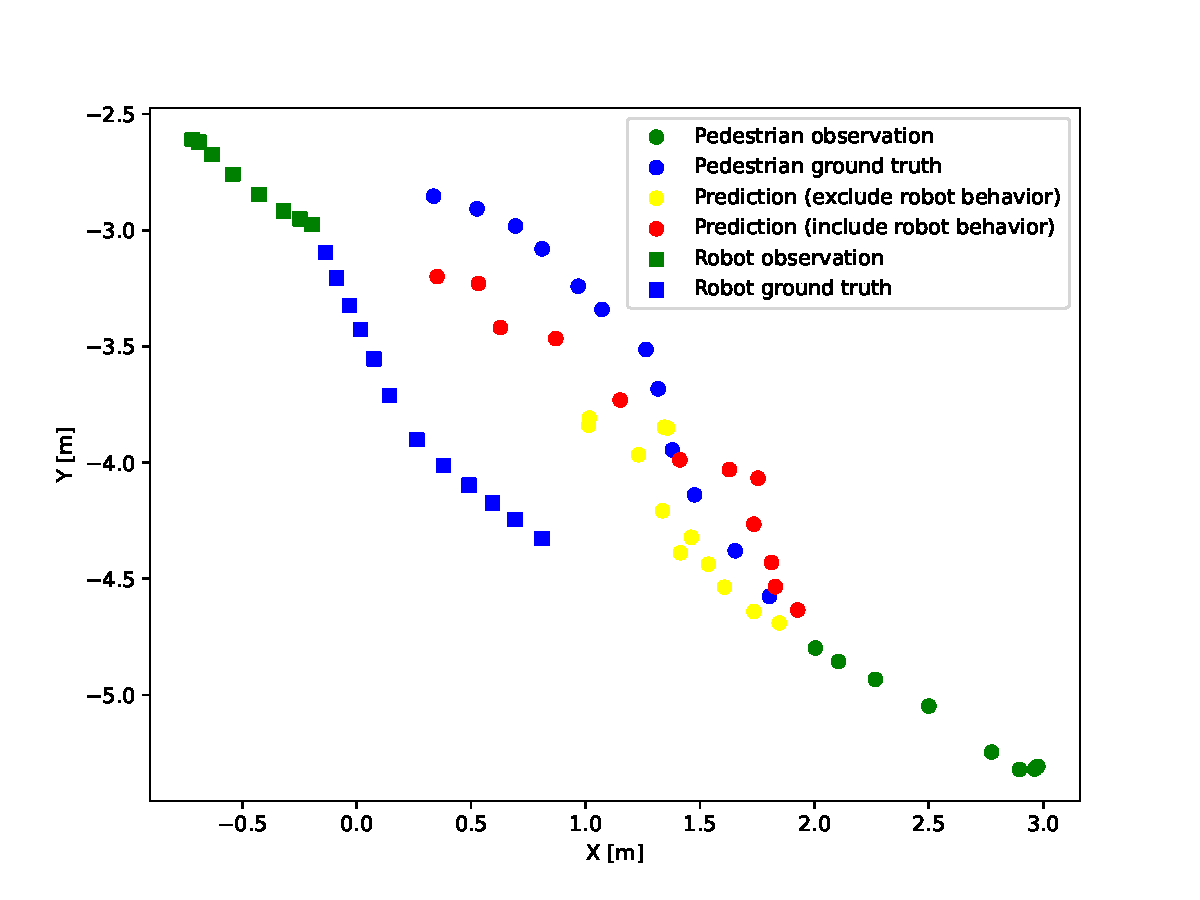
\includegraphics[keepaspectratio, scale=0.58]
      {images/pred_right.pdf}
\caption{Predicted trajectory when the robot moves right}
 \label{Fig:pred-right}
\end{figure}

\vspace{-30pt}

\begin{figure}[H]
  \centering
 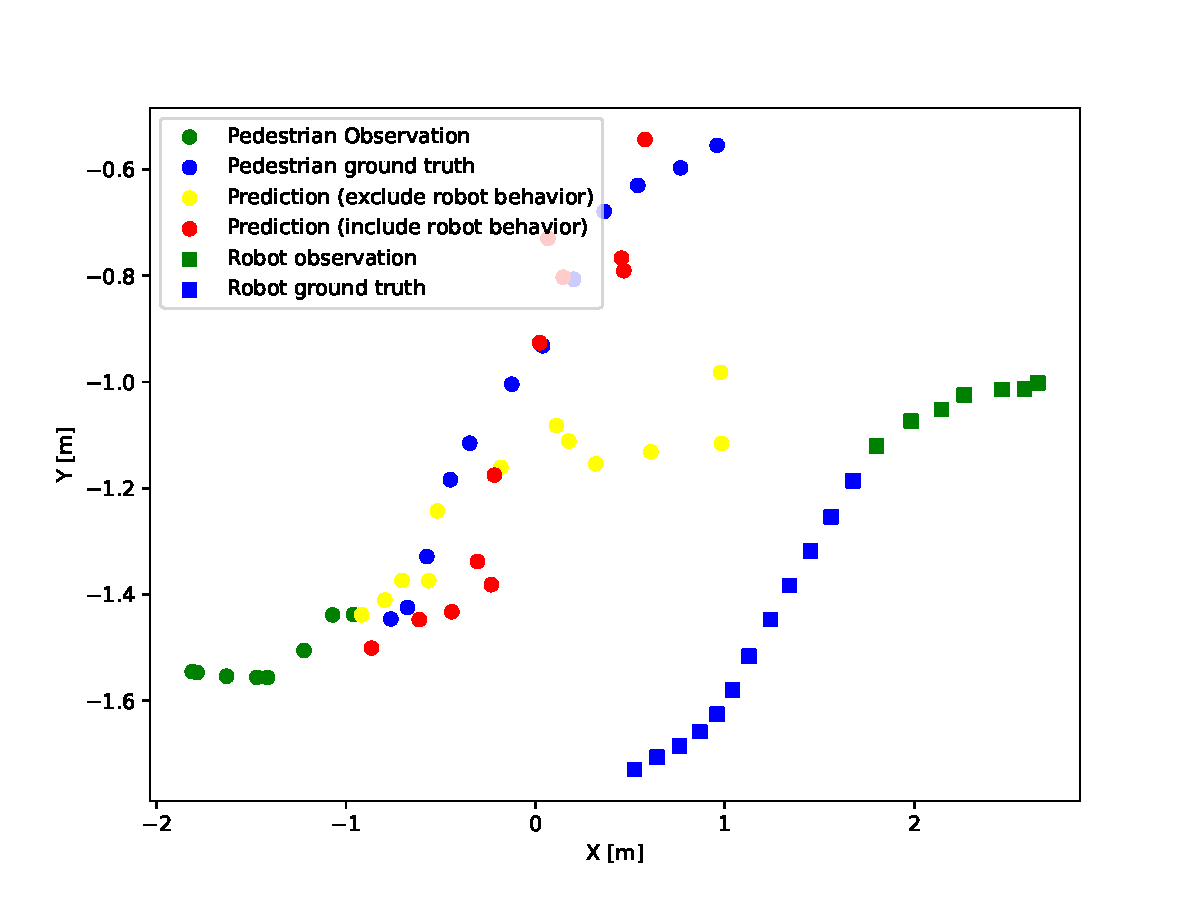
\includegraphics[keepaspectratio, scale=0.58]
      {images/pred_left.pdf}
\caption{Predicted trajectory when the robot moves left}
 \label{Fig:pred-left}
\end{figure}

\newpage
